\documentclass{article}
\usepackage[utf8]{inputenc}
\usepackage{tikz}
\usepackage{geometry}
\geometry{verbose,tmargin=1cm,bmargin=1cm,lmargin=3cm,rmargin=3cm}

\begin{document}
\begin{center}
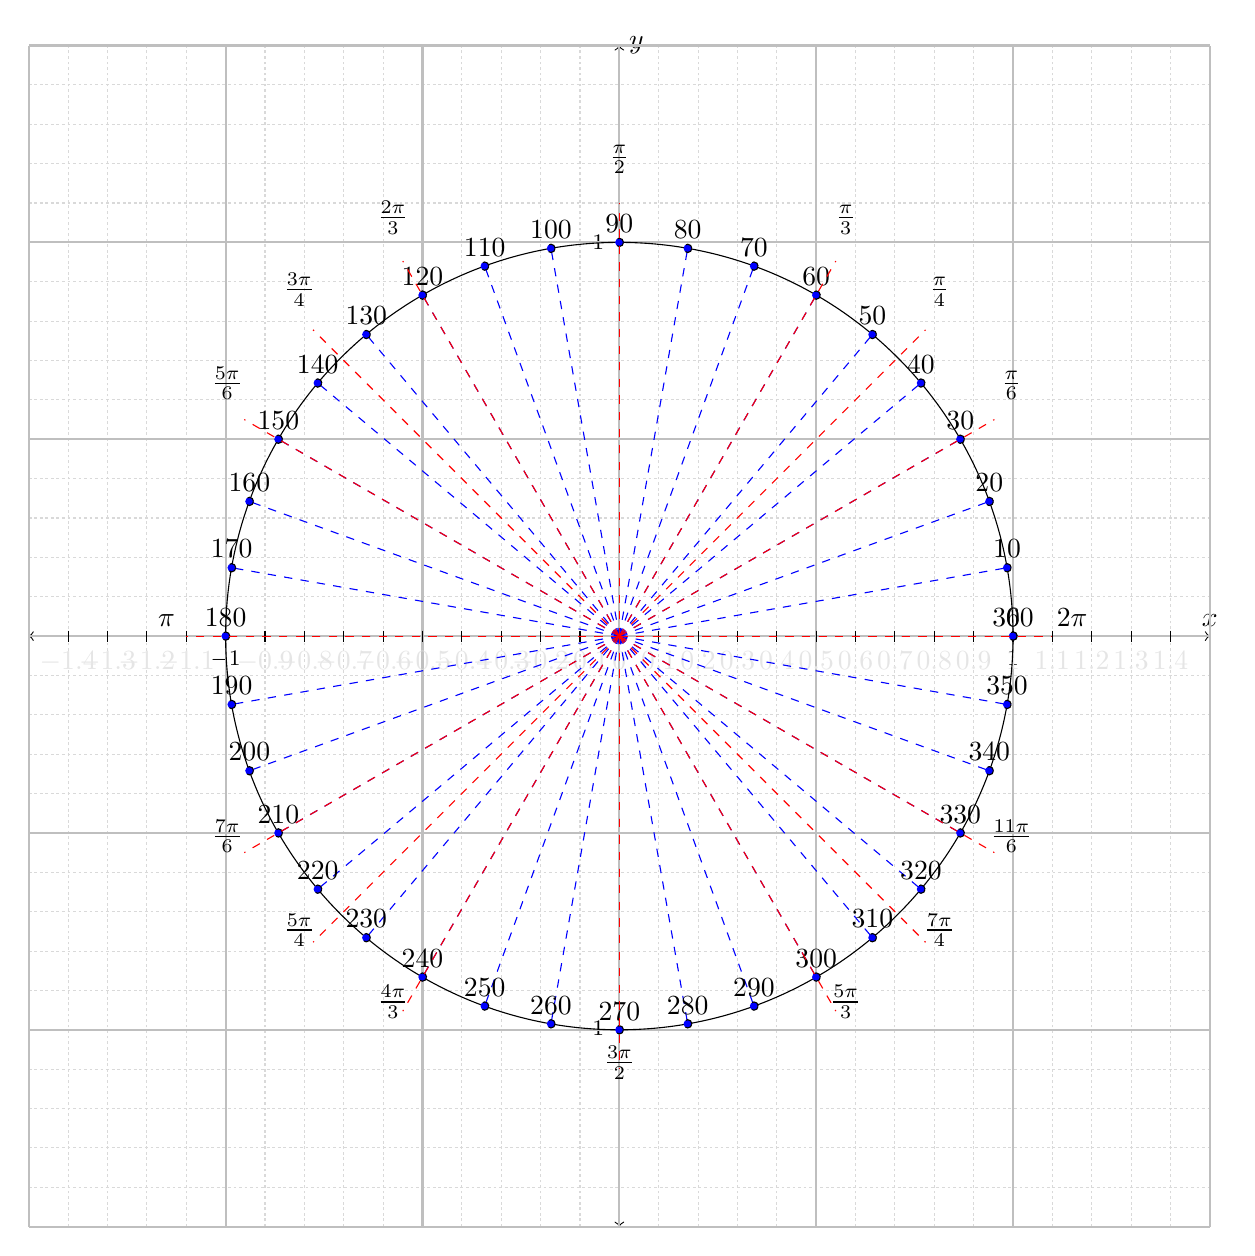
\begin{tikzpicture}[x=5cm,y=5cm]
    \draw[<->] (-1.5,0)--(1.5,0)node[above]{$x$};
    \draw[<->] (0,-1.5)--(0,1.5)node[right]{$y$};

    \foreach \x in {-1,1}
        \draw[shift={(\x,0)}](0pt,2pt)--(0,-2pt)node[below]{\footnotesize $\x$};

    \foreach \y in {-1,1}
        \draw[shift={(0,\y)}](2pt,0pt)--(-2pt,0pt)node[left]{\footnotesize $\y$};
    \draw [color=gray!30,dash pattern=on 1pt off 1pt, xstep=0.1,ystep=0.1] (-1.5,-1.5) grid (1.5,1.5);
    \draw[thick,gray!50,xstep=0.5,ystep=0.5](-1.5,-1.5) grid (1.5,1.5);
    \foreach \x in {-1.4,-1.3,-1.2,-1.1,-0.9,-0.8,-0.7,-0.6,-0.5,-0.4,-0.3,-0.2,-0.1,0,0.1,0.2,0.3,0.4,0.5,0.6,0.7,0.8,0.9,1,1.1,1.2,1.3,1.4}
     \draw(\x,2pt)--(\x,-2pt)node[below,gray!20]{$\x$};
     %\draw[shift={(\x,0)}](0pt,2pt)--(0,-2pt)node[color=gray,rotate=90]{\footnotesize $\x$};

    %\foreach \y in {-1.4,-1.3,-1.2,-1.1,-0.9,-0.8,-0.7,-0.6,-0.5,-0.4,-0.3,-0.2,-0.1,0,0.1,0.2,0.3,0.4,0.5,0.6,0.7,0.8,0.9,1,1.1,1.2,1.3,1.4}
    %    \draw(\y,0)node[below,gray!30]{$\y$};
        %\draw[shift={(0,\y)}](2pt,0pt)--(-2pt,0pt)node[color=gray,left]{\footnotesize $\y$};

    \draw (0,0) circle (1);

    \foreach \x in {0,10,...,360}
        \draw[dashed,color=blue] (0,0)--(\x:1);
    \foreach \x in {0,10,...,360}
        \draw [dashed,fill=blue] (\x:1) circle (1.5pt)node[sloped,above]{$\x$};

    \foreach \x/\xtext in {             
        30/\frac{\pi}{6},             
        45/\frac{\pi}{4},             
        60/\frac{\pi}{3},             
        90/\frac{\pi}{2},             
        120/\frac{2\pi}{3},             
        135/\frac{3\pi}{4},             
        150/\frac{5\pi}{6},             
        180/\pi,             
        210/\frac{7\pi}{6},             
        225/\frac{5\pi}{4},             
        240/\frac{4\pi}{3},             
        270/\frac{3\pi}{2},             
        300/\frac{5\pi}{3},             
        315/\frac{7\pi}{4},             
        330/\frac{11\pi}{6},             
        360/2\pi
        }                 
        \draw (\x:5.75cm) node[above] {$\xtext$};
    \foreach \x in {0,30,...,360}
        \draw[dashed,color=red] (0,0)--(\x:5.5cm);
    \foreach \x in {0,45,...,360}
        \draw[dashed,color=red] (0,0)--(\x:5.5cm);
\end{tikzpicture}
\end{center}
\end{document}

